\section{Setoolkit und Windows 7}
In dieser Aufgabe wurde eine Malware für einen Angriff auf Windows 7 mit dem Setoolkit erzeugt und ausgeführt.

\subsection{Malware mit Veil erzeugen}
Im ersten Schritt musste die E-Mail des Admins gefunden werden. Dies war über einen einfachen telnet Befehl möglich, da die gesuchte Mail als Hilfe hinterlegt war.

\begin{figure}[H]
	\centering
	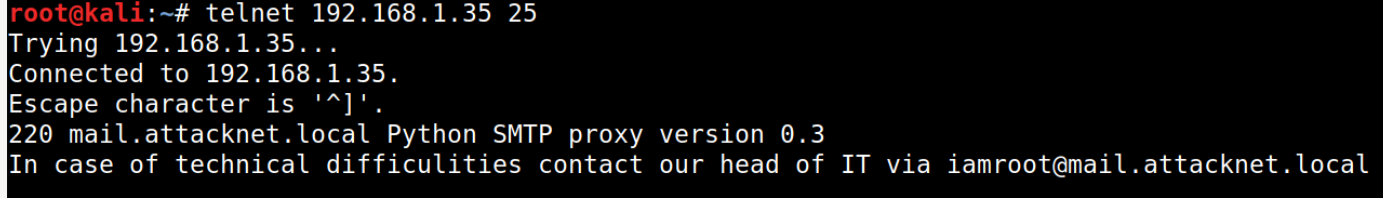
\includegraphics[width=0.85\linewidth]{Whakaahua/aufgabe3/admin_mail.png}
	\caption{Admin Mail}
	\label{fig:admin_mail_3}
\end{figure}

\subsection{Veil}
Im nächsten Schritt wurde mit Veil die Malware erzeugt und anschließend mit VirusTotal überprüft. Die Malware wurde mit Veil erzeugt. Im Programm wurde eine Übersicht der Tools angezeigt.

\begin{figure}[H]
	\centering
	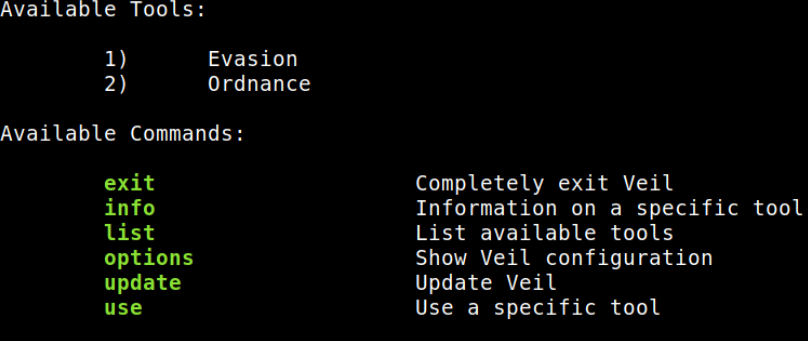
\includegraphics[width=0.85\linewidth]{Whakaahua/aufgabe3/veil1.png}
	\caption{Übersicht}
	\label{fig:veil1}
\end{figure}

Anschließend wurde das Tool Evasion ausgewählt.

\begin{figure}[H]
	\centering
	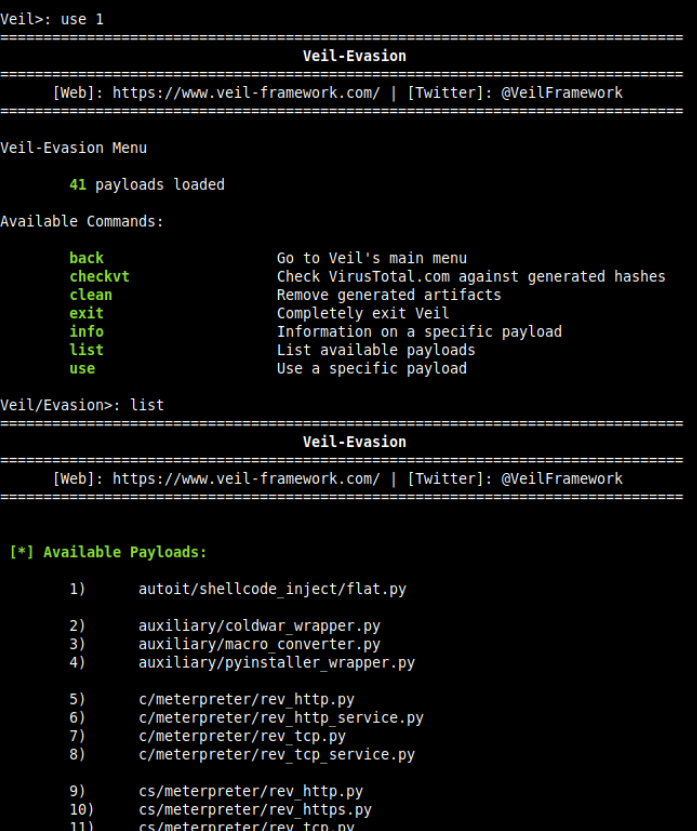
\includegraphics[width=0.85\linewidth]{Whakaahua/aufgabe3/veil2.png}
	\caption{Auswahl des Tools}
	\label{fig:veil2}
\end{figure}

Mit list konnten verschiedene Payloads angezeigt werden. Das Ziel ist es eine Meterpretersession auf dem Zielsystem mittels einer reverse\_shell zu öffnen. Also wurde das passende Payload dafür ausgewählt. In diesem wurden noch der LHOST gesetzt.

\begin{figure}[H]
	\centering
	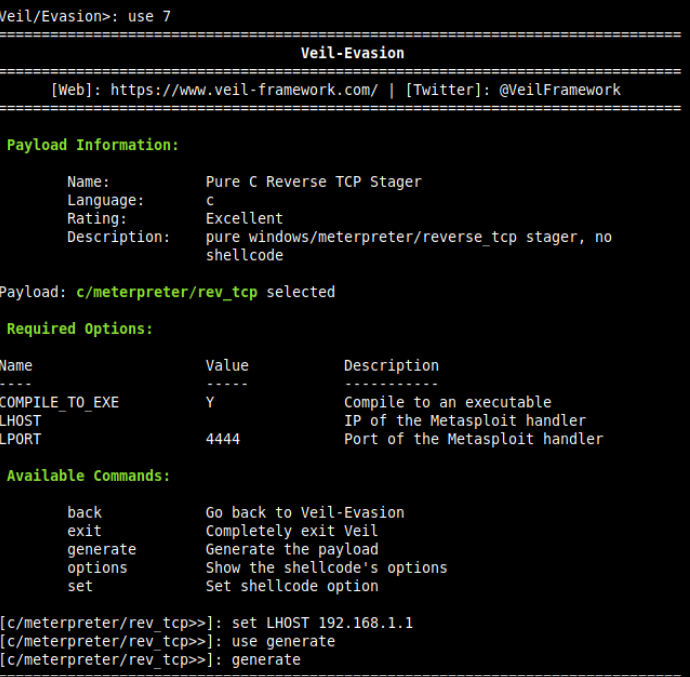
\includegraphics[width=0.85\linewidth]{Whakaahua/aufgabe3/veil3.png}
	\caption{Auswahl des Payloads}
	\label{fig:veil3}
\end{figure}

Im letzten Schritt wurde die Malware mit generate erzeugt.

\begin{figure}[H]
	\centering
	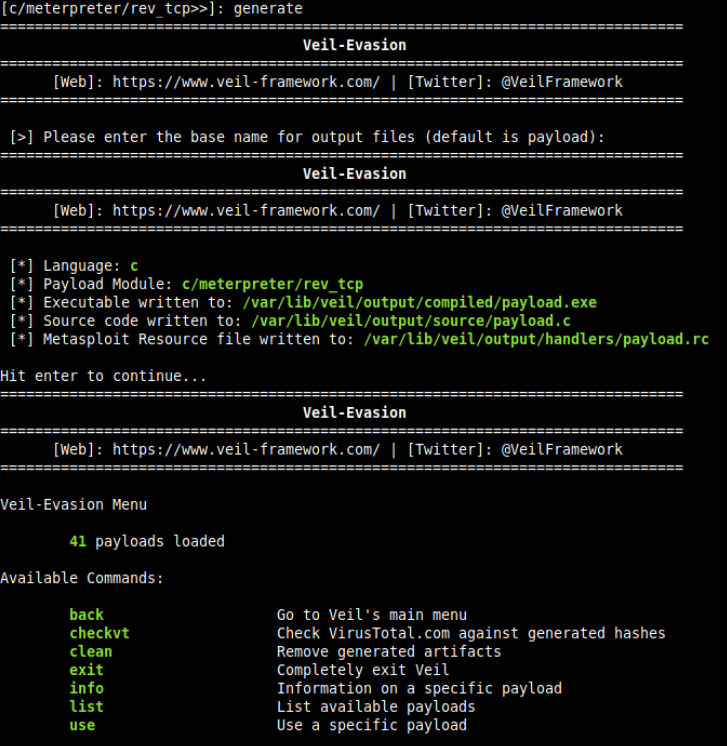
\includegraphics[width=0.85\linewidth]{Whakaahua/aufgabe3/veil4.png}
	\caption{Generierung der Malware}
	\label{fig:veil4}
\end{figure}

Die erzeugte Malware wurde auf VirusTotal getestet. Dabei war zu erkennen, dass nicht alle Virenscanner die Malware auch als solche erkannten. Die Verschleierung war also weitestgehend erfolgreich.

\begin{figure}[H]
	\centering
	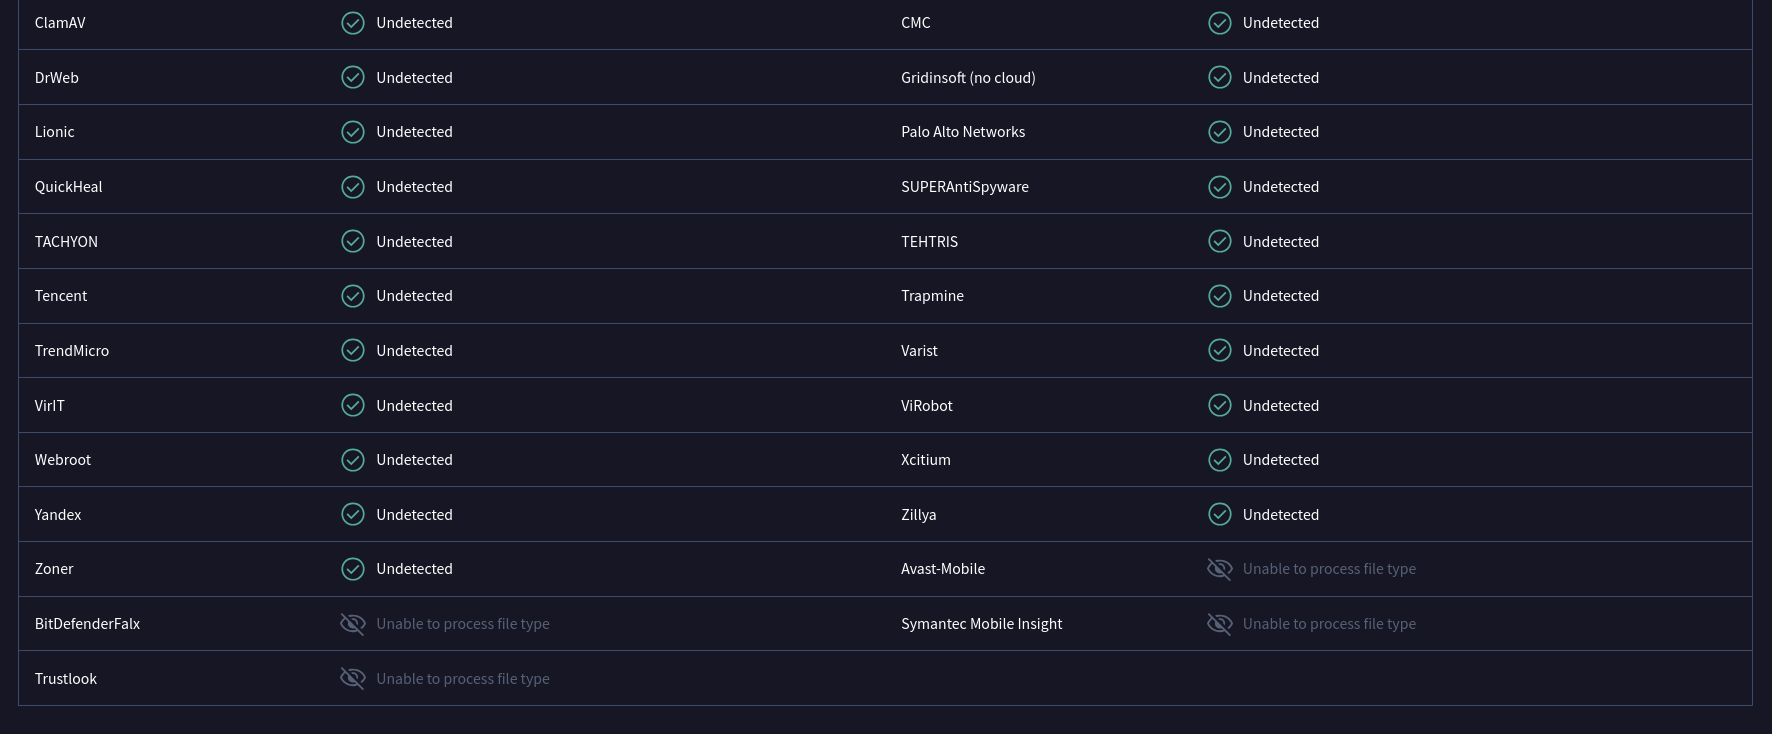
\includegraphics[width=0.85\linewidth]{Whakaahua/aufgabe3/undetected_baaaaam.png}
	\caption{VirusTotal}
	\label{fig:virustotal}
\end{figure}

Die Malware wurde dann per Mail versendet. Falls das Opfer die Datei Öffnet, wird der Angriff gestartet. Unsere Strategie bestand daraus die Malware als Bilder von süßen Hundewelpen zu tarnen. Der Versand der Mail wurde mit swaks gemacht.

\begin{figure}[H]
	\centering
	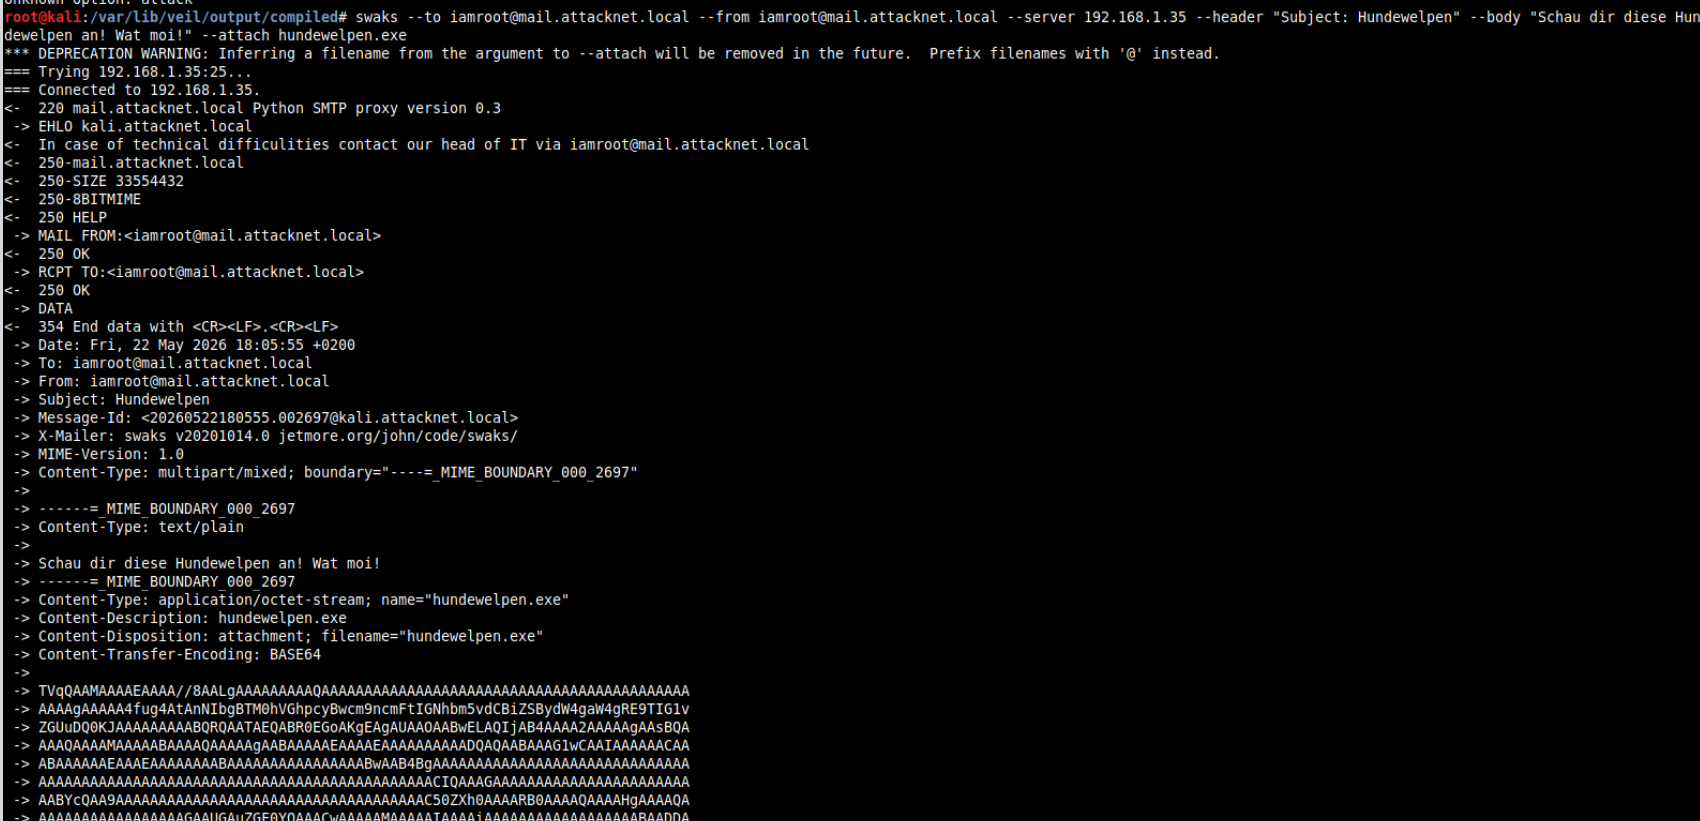
\includegraphics[width=0.85\linewidth]{Whakaahua/aufgabe3/send_mail_attack_swaks.png}
	\caption{Mail mit Malware versenden}
	\label{fig:virustotal}
\end{figure}

Auf unserem System wurde über meterpreter eine reverse\_tcp Verbindung gestartet.

\begin{figure}[H]
	\centering
	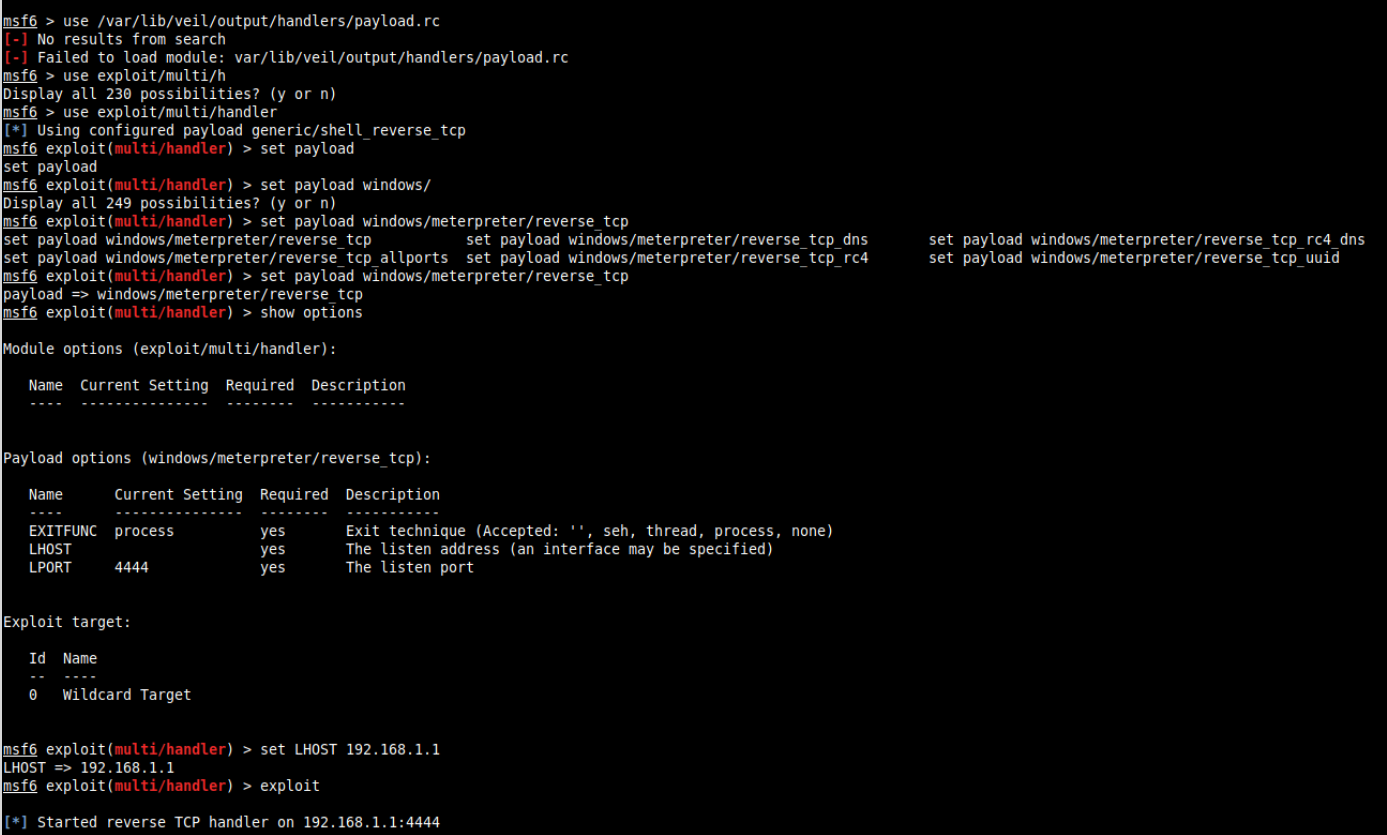
\includegraphics[width=0.85\linewidth]{Whakaahua/aufgabe3/start_listening.png}
	\caption{reverse\_tcp}
	\label{fig:listen}
\end{figure}

Anschließend wurde der exloit ausgeführt und ein Screenshot als Erfolg angefertigt.

\begin{figure}[H]
	\centering
	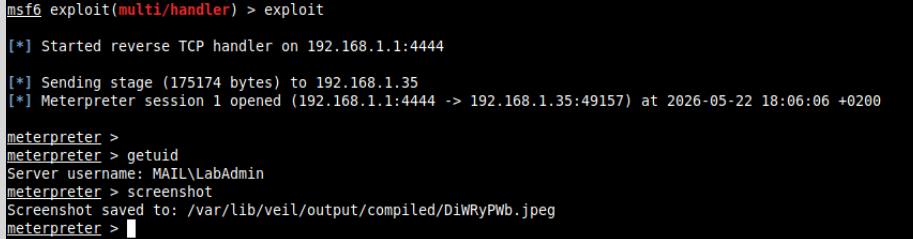
\includegraphics[width=0.85\linewidth]{Whakaahua/aufgabe3/success_heurika.png}
	\caption{Erfolg}
	\label{fig:erfolg_3}
\end{figure}

\subsection{Credential Harvester Attack}
Im allgemeinen geht es bei einer Credential Harvester Attack darum, Anmeldedaten für einen Dienst zu klauen. Das kann unter anderem mit einer gefälschten Website geschehen. Als Beispiel könnte eine Kopie einer Bankseite unter einer ähnlichen Domain veröffentlicht werden (z.B. spar-kasse.de anstatt sparkasse.de) Auf diese Seite werden dann Opfer z.B. mittels Phishing gelockt und angefordert sich anzumelden. Diese Daten kann dann der Angreifer in einer Datenbank speichern. Somit hat der Angreifer wahrscheinlich gültige Anmeldedaten bekommen. Dieses Vorgehen wurde mit einer Kopie von Moodle gezeigt. Mit dem Setoolkit ist es möglich eine Website zu klonen und diese lokal zu hosten. Als erstes wurde dazu Moodle mit dem entsprechenden Tool geklont. Im Anschluss war die Seite auch über Localhost bzw. über die entsprechende IP auch von andern Rechnern aus dem selben Netz erreichbar.

\begin{figure}[H]
	\centering
	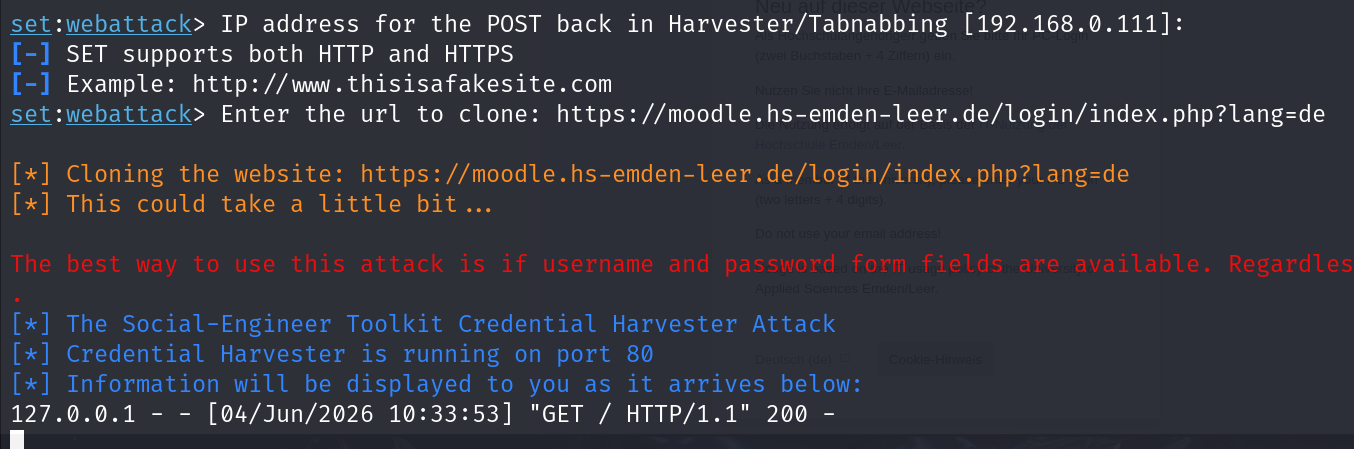
\includegraphics[width=0.85\linewidth]{Whakaahua/aufgabe3/moodle_clone_pics/setoolkit_webclonee_attack_start.png}
	\caption{Klonen einer Website mit dem SET}
	\label{fig:Klonen einer Website mit dem SET}
\end{figure}

Nachdem Moodle erfolgreich geklont wurde, konnte die Seite begutachtet und auf Fehler untersucht werden.

\begin{figure}[H]
	\centering
	
	\begin{subfigure}{0.48\textwidth}
		\centering
		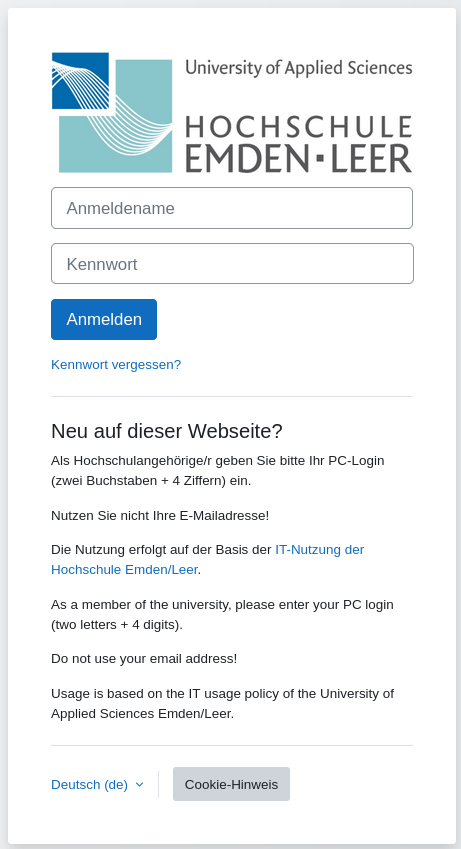
\includegraphics[width=\linewidth]{Whakaahua/aufgabe3/moodle_clone_pics/moodle_login_original.png}
		\caption{Original Login}
		\label{fig:moodel orig}
	\end{subfigure}
	\hfill
	\begin{subfigure}{0.48\textwidth}
		\centering
		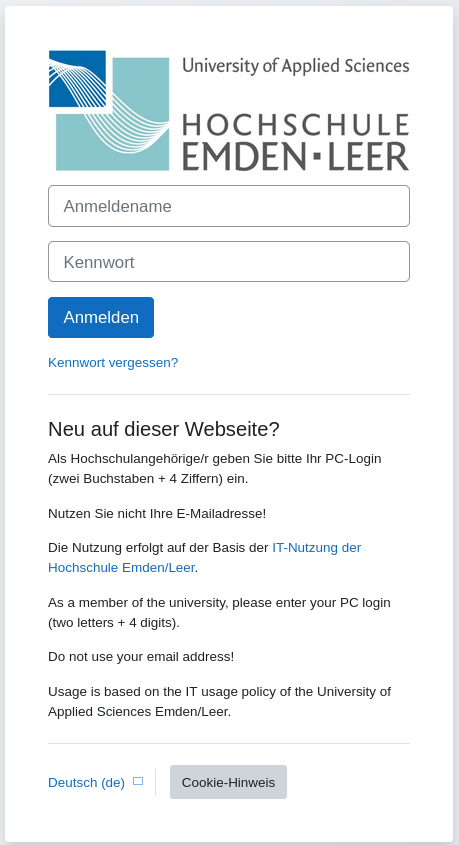
\includegraphics[width=\linewidth]{Whakaahua/aufgabe3/moodle_clone_pics/moodle_login_cloned.png}
		\caption{Geklonter Login}
		\label{fig:moodle clone}
	\end{subfigure}
	
	\caption{Vergleich der Login Seiten}
	\label{fig:vergleich}
\end{figure}

\begin{figure}[H]
	\centering
	
	\begin{subfigure}{0.48\textwidth}
		\centering
		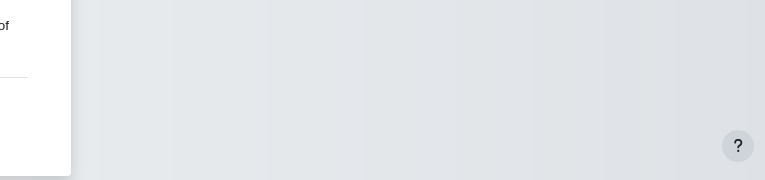
\includegraphics[width=\linewidth]{Whakaahua/aufgabe3/moodle_clone_pics/moodle_login_original_questionmark.png}
		\caption{Original Fragezeichen}
		\label{fig:moodel frag}
	\end{subfigure}
	\hfill
	\begin{subfigure}{0.48\textwidth}
		\centering
		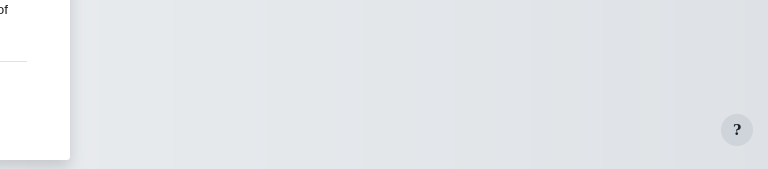
\includegraphics[width=\linewidth]{Whakaahua/aufgabe3/moodle_clone_pics/moodle_login_cloned_questionmark.png}
		\caption{Geklontes Fragezeichen}
		\label{fig:moodle clone frag}
	\end{subfigure}
	
	\caption{Vergleich der Login Seiten}
	\label{fig:vergleich}
\end{figure}

Es gibt zwei Unterschiede, die allerdings nur bei genauer Betrachtung auffallen und im 1 zu 1 Vergleich. Es wird ein Icon nicht angezeigt und das Fragezeichen ist auf der Geklonten Seite anders. Das sind allerdings kleine Details, welche bei einem schnellen anmelden nicht auffallen würden. Etwas auffälliger ist die Fehlermeldung, welche beim betreten der Seite angezeigt wird. Allerdings würde diese Fehlermeldung im Alltag einfach als ein kleiner technischer defekt abgeschrieben werden und unwahrscheinlich als Zeichen einer gefälschten Website wahrgenommen werden.

\begin{figure}[H]
	\centering
	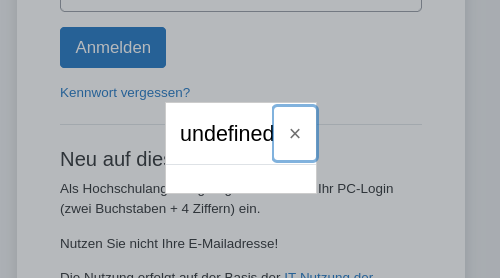
\includegraphics[width=0.85\linewidth]{Whakaahua/aufgabe3/moodle_clone_pics/moodle_login_cloned_undefined.png}
	\caption{Fehlermeldung}
	\label{fig:Klonen fehlermeldung}
\end{figure}


Zusammenfassend lässt sich die gefälschte Website nur sehr schwer erkennen und erfordert ein geschultes Auge. Am ehesten lässt sich dies wahrscheinlich anhand der URL erkennen (gut das unser Rechenzentrum die URL geändert hat).
